\documentclass[tikz,border=2mm]{standalone}
\usepackage{tkz-euclide}
\usepackage{fp}

% side length of the square
\edef\s{1}

% diagonal length of the square
% \edef\d{\fpeval{1.41421356*\s}}
\edef\d{\fpeval{sqrt(2)*\s}}

% radius of the circle
\edef\r{\fpeval{0.3}}
%\edef\r{\fpeval{5/9}}

% coordinates of center of circle
%\edef\e{\fpeval{\s+\r}}
\edef\e{\fpeval{\s-\r}}

\begin{document}
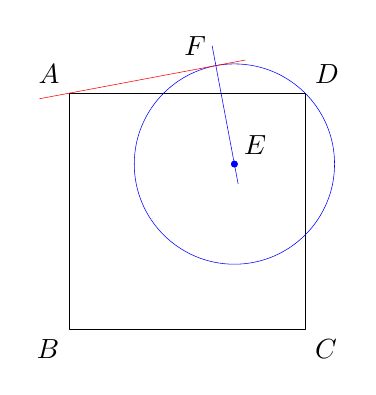
\begin{tikzpicture}[scale=3]
  % draw the square
  \tkzDefPoint(0,\s){A} 
  \tkzDefPoint(0,0){B} 
  \tkzDefPoint(\s,0){C} 
  \tkzDefPoint(\s,\s){D}
  \tkzDrawPolygon(A,B,C,D)
  
  % draw the circle 
  \tkzDefPoint(\e,\e){E} 
  \tkzDrawPoint[color=blue](E)
  \tkzDrawCircle[color=blue](E,D)
  \tkzDrawPoint[color=blue](E)

  % label the points
  \tkzLabelPoints[above left](A)
  \tkzLabelPoints[below left](B)
  \tkzLabelPoints[below right](C)
  \tkzLabelPoints[above right](D)
  \tkzLabelPoints[above right](E)

  % get the tangent
  \tkzDefLine[tangent from=A](E,D)\tkzGetPoints{F}{G}
  \tkzLabelPoints[above left](F)
  \tkzDrawLines[color=red](A,F)
  \tkzDrawLines[color=blue](E,F)
\end{tikzpicture}
\end{document}
